\section{Results and Analysis}
%
The results in this section was obtained by running the program \verb+poisson-mpi.c+ on the Kongull cluster. To reproduce the results the environment should be set by sourcing \verb+environment.sh+ and compiled using \verb+compileKongull.sh+. Each job was submitted individually to a batch queue, and all jobs can be run with \verb+results.sh+. All the plots can then be generated by running \verb+plotting.R+.
%
\subsection{Convergence analysis}
First it is important to verify that the code works correctly. This was done by comparing the results to an analytical solution and plotting the error for different problem sizes $n$. The loading function chosen for this task was 
\begin{align}
  \label{eq:conv} 
  f = 5 \pi^2 \sin (\pi x) \sin (2 \pi y),
\end{align}
with the solution
\begin{align}
  u = \sin (\pi x) \sin (2 \pi y). 
\end{align}
The max norm was used to measure the error. The calculations were run with two threads on 1, 3 and 6 MPI processes, and the results can be found in Figure~\ref{fig:errVsn}. This plot is a log-log plot, with a reference line of slope $-2$. As the points follow the line, this means the method has quadratic convergence. As the numerical scheme is a second order method, the figure confirms that our implementation is correct. For the rest of this section all tests are done with the $f$ in Eq.~\eqref{eq:conv}, unless specified otherwise.\\
%
\begin{figure}[h!]
\begin{center}
    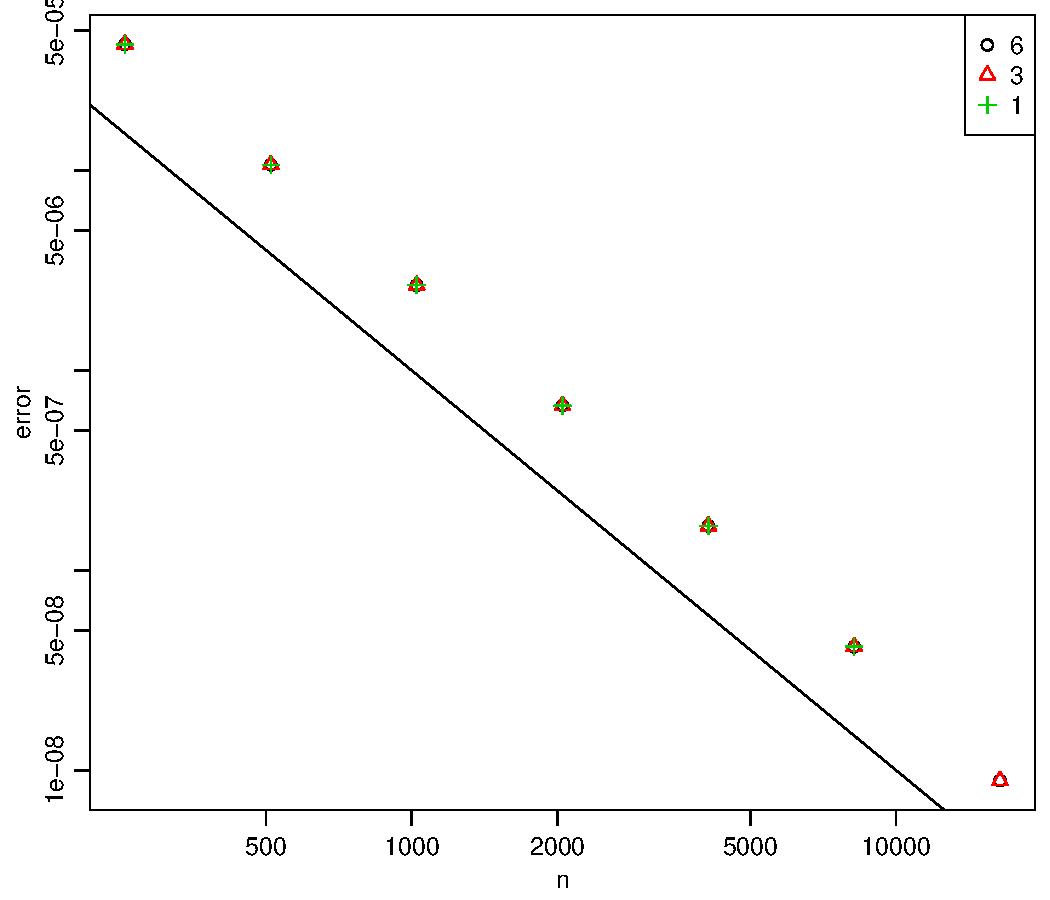
\includegraphics[scale=0.4]{./Figures/errVsn.pdf}
\end{center}
  \vspace{-1\baselineskip}
\caption{Loglog plot of the error as function of $n$. A reference line with slope $-2$ is drawn. The problem is run on two threads with the number of MPI processes specified in the legend.}
\label{fig:errVsn}
\end{figure}
%
\\
\subsection{Shared or distributed memory models}
In order to show the difference between shared and distributed memory parallelization the problem was runned on a single node where all 12 processors were utilized. The point was to investigate the performance of using threads versus MPI processes. Thus the relation between threads $t$ and MPI processes $p$ is $p t = 12$ or $p = 12/t$. The calculations were done with $n = 2^{14} = 16384$. 
The same problem was repeated on three nodes where all 12 processors were utilized in the same way as above. The results can be found in Figure~\ref{fig:taskc}. It is clear from this figure that the time varies from each time the code is runned. This is important to take into account later in the report, where the problem is only run once for each test case. It is clear from both plots that it is preferable to use only MPI processes and no openMP. 

While running only one MPI process and 12 threads on one node there is still some overhead from the MPI sending to itself and the work of reordering the data. Therefore the problem was solved on 12 threads without this overhead. The results are the red crosses in Figure~\ref{fig:taskc}. It is clear that it is a lot faster than with the MPI sending, but it is still slower than running with 12 MPI processes. 

The reasons for why pure MPI code is faster than the hybrid and even the pure openMP are most likely that the optimalization done by the compilator is better developed for the MPI library than for openMP. The overhead cost related to creating and closing threads are a lot higher than dividing the node into MPI processes. The advantage openMP has over MPI is the fact that all threads shares memory, instead of distributing memory to each process. Thus openMP is advantageous over MPI if the problem requires that many processors uses the same memory. Since our problem has a relative small memory usage, and the communication needed between the processors is minimal (only two send operations of $8n^2$ bytes is required) pure MPI is the optimal way to parallelize the code.  
\\
\begin{figure}[h!]
  \centering
  \begin{subfigure}[b]{0.48\textwidth}
    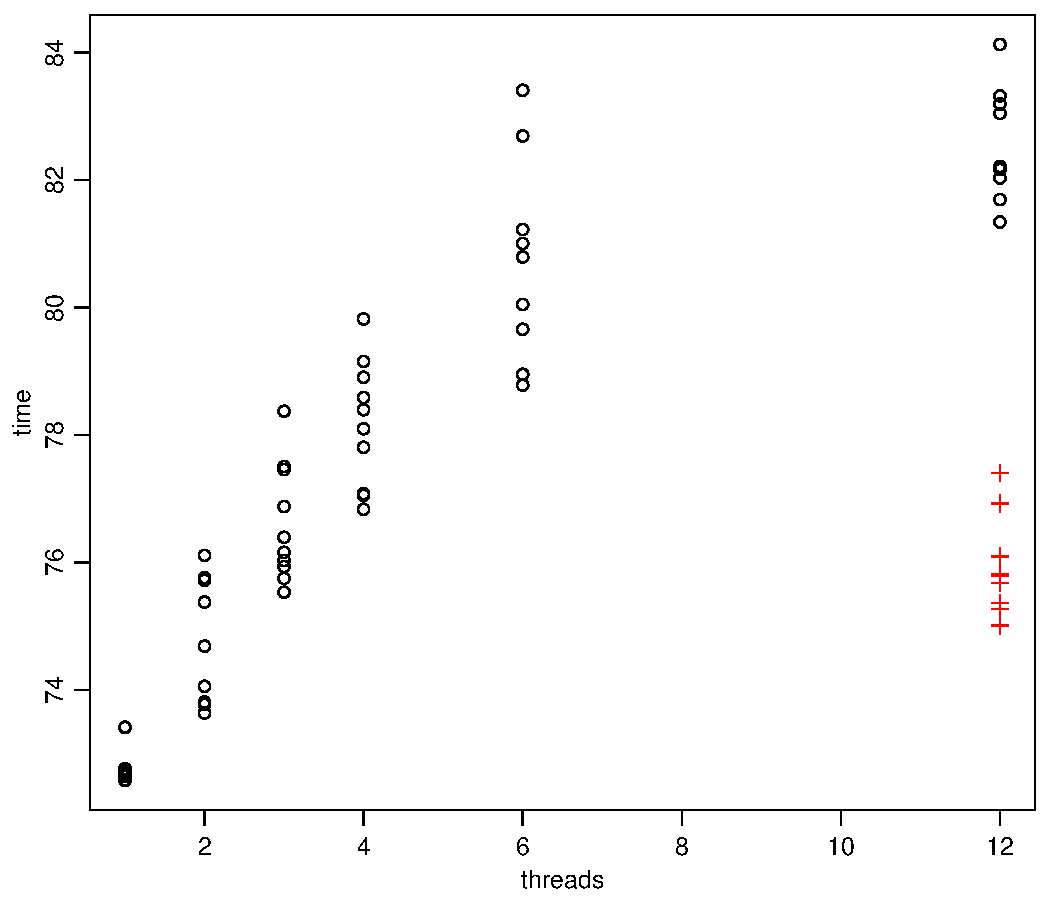
\includegraphics[width=\textwidth]{./Figures/taskc1.pdf}
  \end{subfigure}%
  \quad
  \begin{subfigure}[b]{0.48\textwidth}
    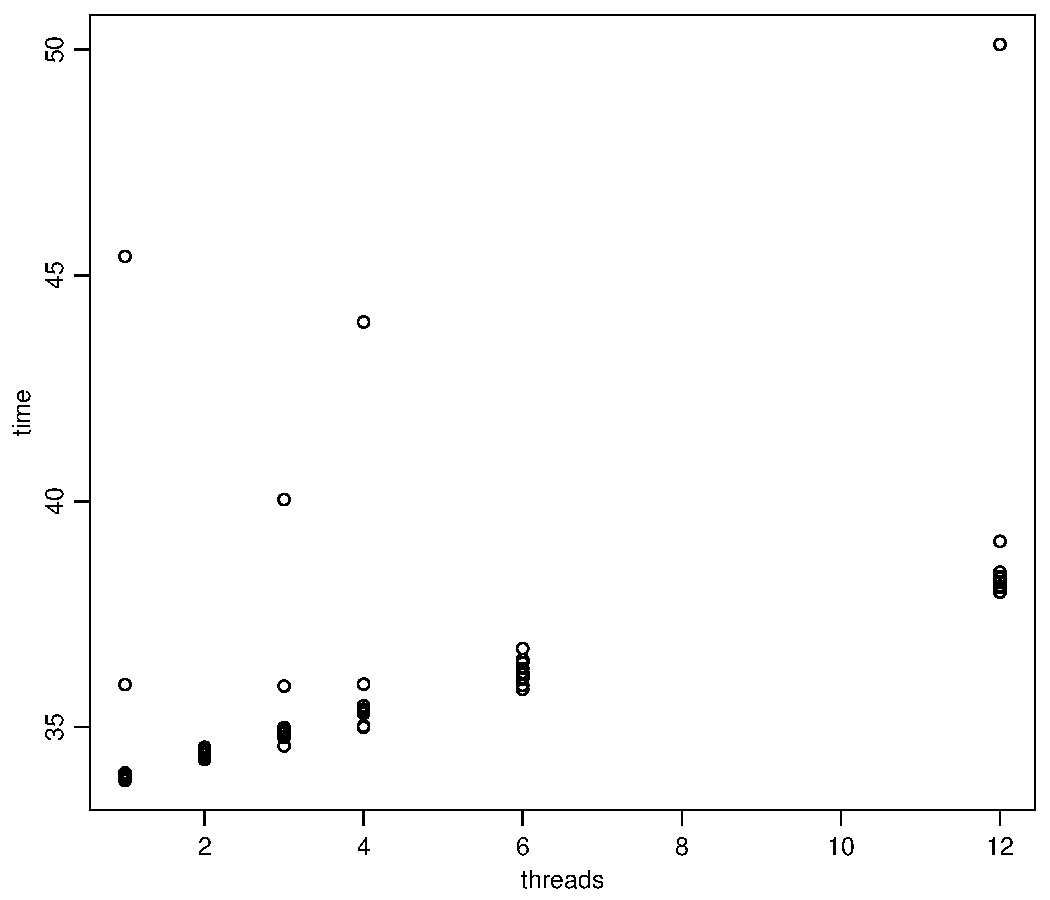
\includegraphics[width=\textwidth]{./Figures/taskc2.pdf}
  \end{subfigure}
          %(or a blank line to force the subfigure onto a new line)
  \vspace{-0.1\baselineskip}
  \caption{Times (in seconds) for running MPI processes vs threads with $n = 2^{14}$. The total number of processors used are 12 per node, so the number of MPI processes per node is $12 / threads$. The left figure is run on one node, while the right is run on three nodes. The red crosses are run without any MPI sending at all.}
  \label{fig:taskc}
\end{figure}
\\
\subsection{Timing results}
\subsubsection{Time as a function of $p$}
Timing results were obtained by running the problem on different number of MPI processes with one thread. Here up to three nodes were used, and a new node was only used when there were no more free processors in the previous nodes. This was done for different problem sizes and plotted in Figure~\ref{fig:time1}. Sending between MPI processes on a single node should be faster than sending between nodes. This trend is clear in the figure, as the first points after utilizing an extra node (after the vertical lines), clearly do not follow the trend of the previous points. 

In Figure~\ref{fig:time2}, the same experiment is done, but with two threads instead of one. So here only up to 6 MPI processes were used on each node. Although it is clear from Figure~\ref{fig:taskc} that this should be worse than only using MPI processes, it is hard to distinguish Figure~\ref{fig:time1} and Figure~\ref{fig:time2}. To investigate how the time changed with only using threads on each node, the problem was run on 1 to 12 threads on 1 to three nodes. In Figure~\ref{fig:time3} this is plotted and we see the behavior is the same as in the other figures. It is reasonable to assume that for if run on more nodes, the time would eventually start to grow because of the overhead. There are some larger times at the end of Figure~\ref{fig:time1}, but this is probably just noise.\\
%
\begin{figure}[h!]
  \centering
  \begin{subfigure}[b]{0.48\textwidth}
    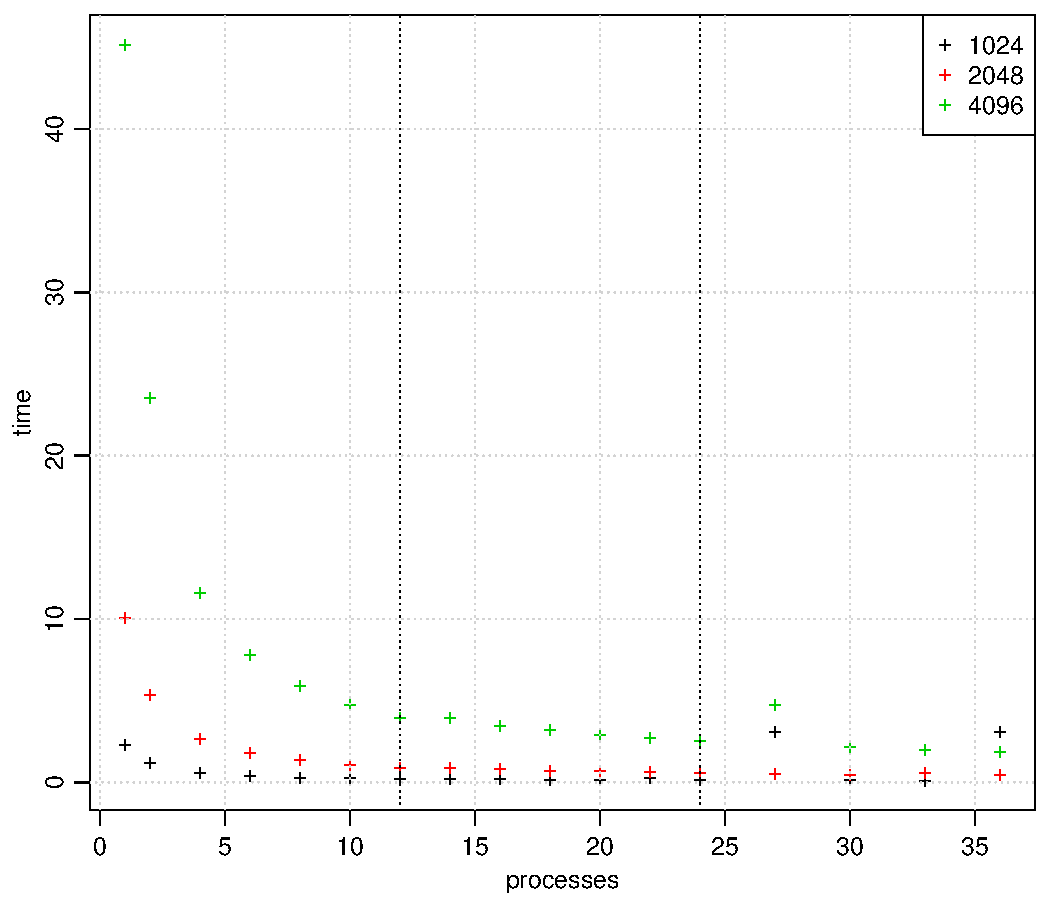
\includegraphics[width=\textwidth]{./Figures/taskbTimeProc1.pdf}
    \caption{}
    \label{fig:time1}
  \end{subfigure}%
  \quad
  \begin{subfigure}[b]{0.48\textwidth}
    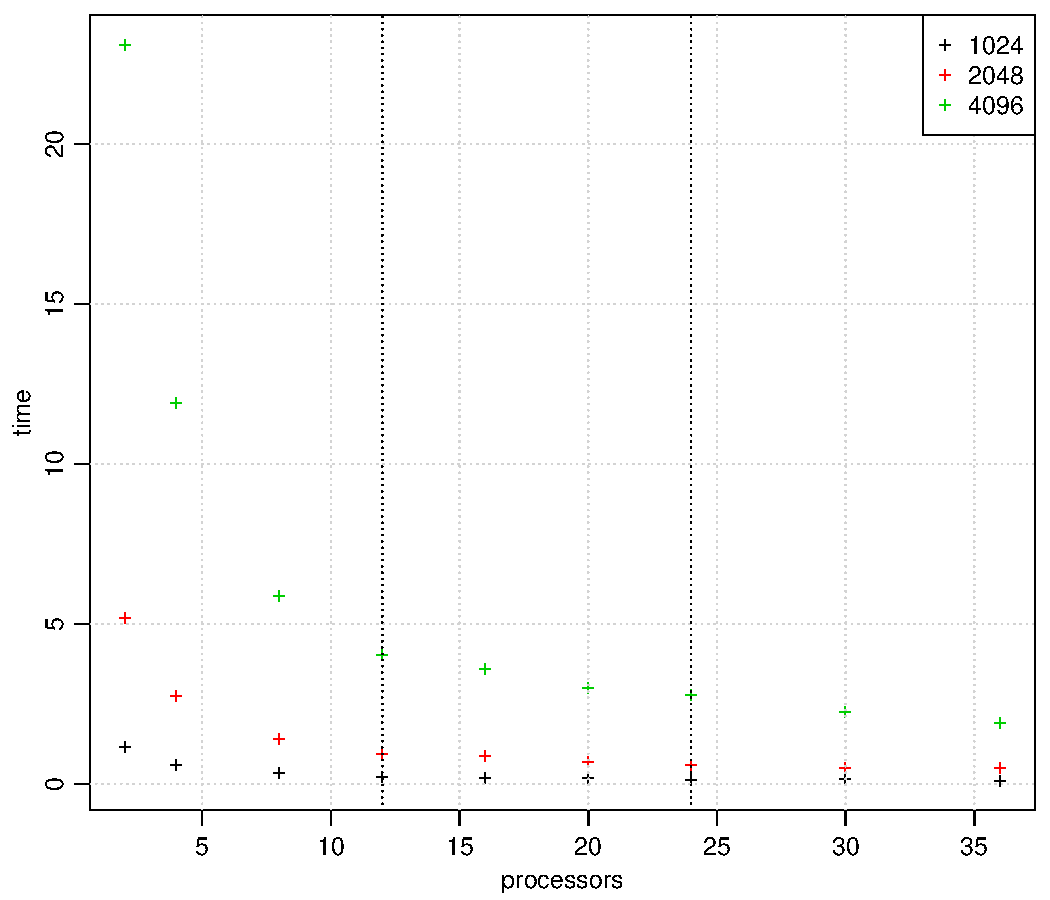
\includegraphics[width=\textwidth]{./Figures/taskbTimeProc2.pdf}
    \caption{}
    \label{fig:time2}
  \end{subfigure}
  \quad
  \begin{subfigure}[b]{0.48\textwidth}
    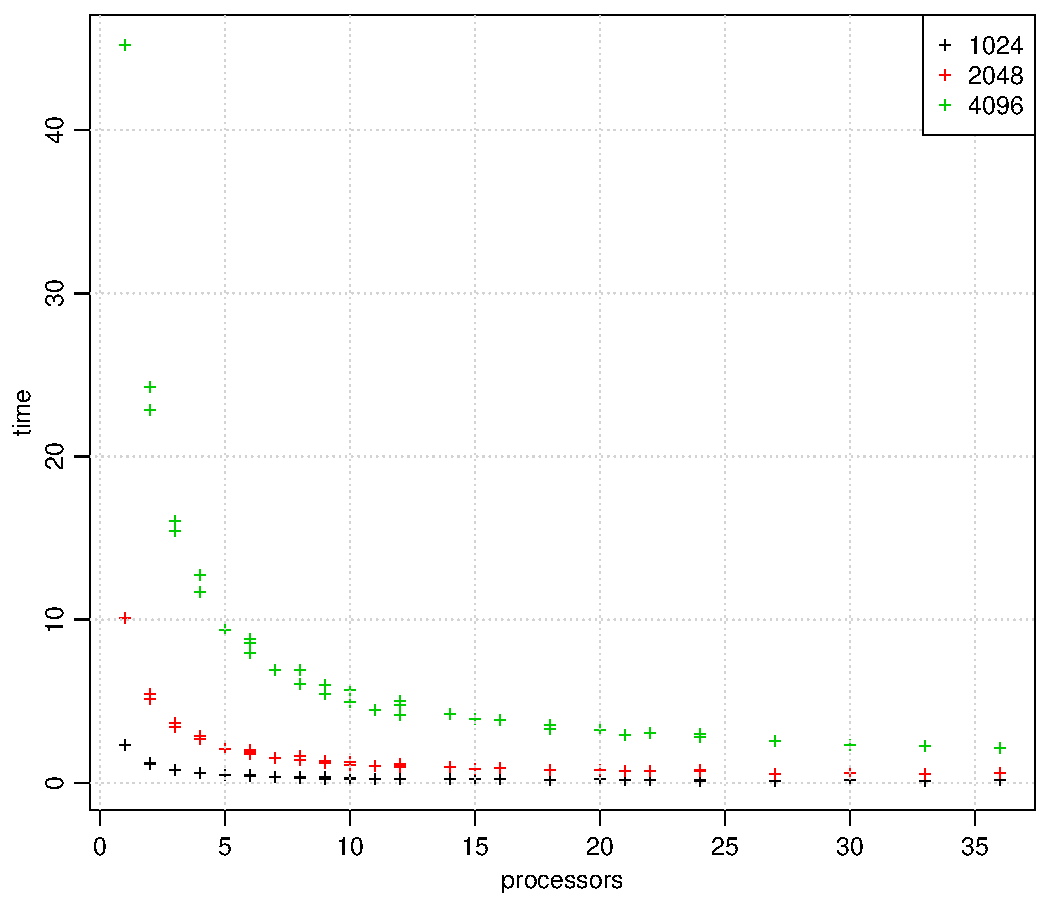
\includegraphics[width=\textwidth]{./Figures/taskbTimeNodesTimesThreads.pdf}
    \caption{}
    \label{fig:time3}
  \end{subfigure}
          %(or a blank line to force the subfigure onto a new line)
  \vspace{-0.1\baselineskip}
  \caption{Times for running problem with different amount of MPI processes. (a) each MPI process has one thread. (b) each MPI process has two threads. (c) One MPI process is run per node, and the number of threads varies from 1 to 12. (all) The problem is run on as few nodes as possible, and the MPI processes are identically distributed among the nodes. The problem size $n$ is specified in the plots. The vertical lines separate the domain to show when 1, 2 and 3 nodes are used.}
  \label{fig:Times}
\end{figure}
%
\\
\subsubsection{Time as a function of $n$}
The time of the algorithm should be of order $O(n^2 \log(n))$. To investigate how the time scales with $n$, $time/n^2$ was plotted as a function of $n$. This is displayed in the left plot in Figure~\ref{fig:timeVsn}. The data used is the same as in Figure~\ref{fig:errVsn}. One can clearly see an upward trend for larger problem sizes due to the factor $log(n)$. Therefore $time/(n^2 \log(n))$ was also plotted in Figure~\ref{fig:timeVsn}. Here the ratio is constant and it can be concluded that the time is of order $O(n^2 \log(n))$. For small times, the overhead becomes significant, and that is probably why the first point is so much higher for 3 and 6 MPI processes. Notice also by studying the slopes in the left plot of figure~\ref{fig:timeVsn} that the impact of the factor $log(n)$ is really small.  
\begin{figure}[h!]
  \centering
  \begin{subfigure}[b]{0.48\textwidth}
    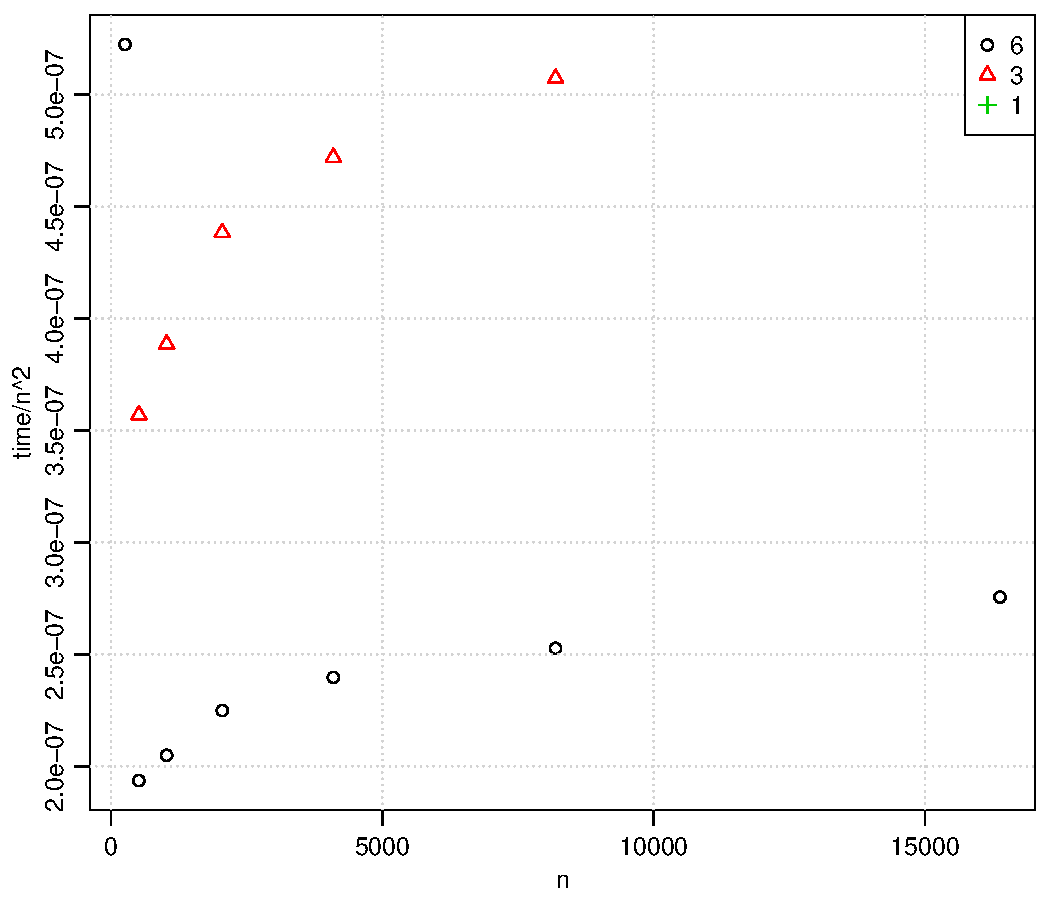
\includegraphics[width=\textwidth]{./Figures/timeOverN2Vsn.pdf}
  \end{subfigure}%
  \quad
  \begin{subfigure}[b]{0.48\textwidth}
    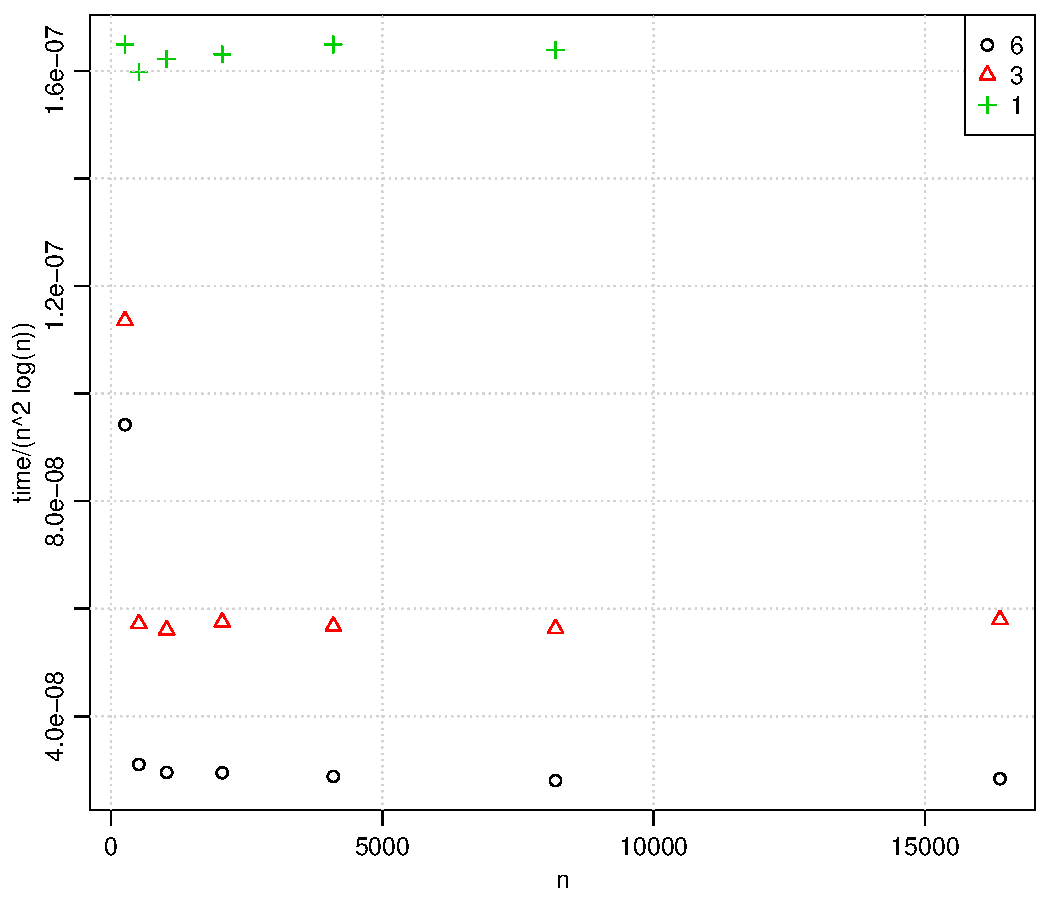
\includegraphics[width=\textwidth]{./Figures/timeOverN2LogNVsn.pdf}
  \end{subfigure}
          %(or a blank line to force the subfigure onto a new line)
  \vspace{-0.1\baselineskip}
  \caption{Left plot is $Time/n^2$ as function of $n$. The right plot is $Time/(n^2 \log (n))$. The data is the same as in Figure~\ref{fig:errVsn}.}
  \label{fig:timeVsn}
\end{figure}
\\
\subsection{Speedup and Efficiency}
While Figure~\ref{fig:Times} displays the times, it is hard to get a lot of information from the plots. A useful diagnostics tool is the speedup $S_p=T_1/T_p$, where $T_p$ is the time used with $p$ processors. If there is perfect speedup, i.e. for $p$ processors the time $T_p = T_1/p$, then the speedup should be a linear function of the nr. of processors, with slope 1. The speedup, along with a reference line of slope 1, is plotted in Figure~\ref{fig:Speedup}.The setup is exacly the same as in Figure~\ref{fig:Times}.

From this plot it is clear that the speedup is better for larger problem sizes. This makes sense as the overhead becomes less significant as the time increases. Also note that there are some noisy points, especially for the smallest problem size. This was addressed in the beginning of this section. What is clear here is that the noise has a higher impact on small problems as the time is shorter, which makes perfect sense. Also here it is clear that there are more overhead when problem is done on one more node (see points after vertical lines in upper left figure). After the last vertical line the time gets really small and the data gets quite noisy.
The trend is nevertheless clear, an increasing amount of nodes decreases the speedup. \\
\\
When sending data between processes with MPI, the speedup is not expected to be 1. By using the \textit{linear network model} \eqref{eq:linNetMod}, a better estimate can be obtained (though still not very accurate).
\begin{align}
  \tau_s(b) &= \tau_c + \gamma b, \notag \\
  \label{eq:linNetMod} 
  T_p &= \frac{T_1}{p} + \tau_s \left(  8 \frac{n^2}{p}\right), \\
  S_p &= \frac{T_1}{T_p}. \notag 
\end{align}
Here $\tau_s$ is the time to communicate $b$ bytes and $\tau_c$ is the latency of the network. In Figure~\ref{fig:Speedup}, the green line is from \eqref{eq:linNetMod}, with $\tau_c = 10^{-6}$ and $\gamma = 5 \cdot 10^{-9}$. The lines seems to be a good approximation for one node, but not for more than one. This makes sense as it takes longer time to send data between nodes than internally in a node.
\\ \colorbox{yellow}{Might want to explain why we send everything once, instead of each column.}\\
\colorbox{yellow}{I think the calculations might suggest to send one col at a time.}
%
\begin{figure}[h!]
  \centering
  \begin{subfigure}[b]{0.48\textwidth}
    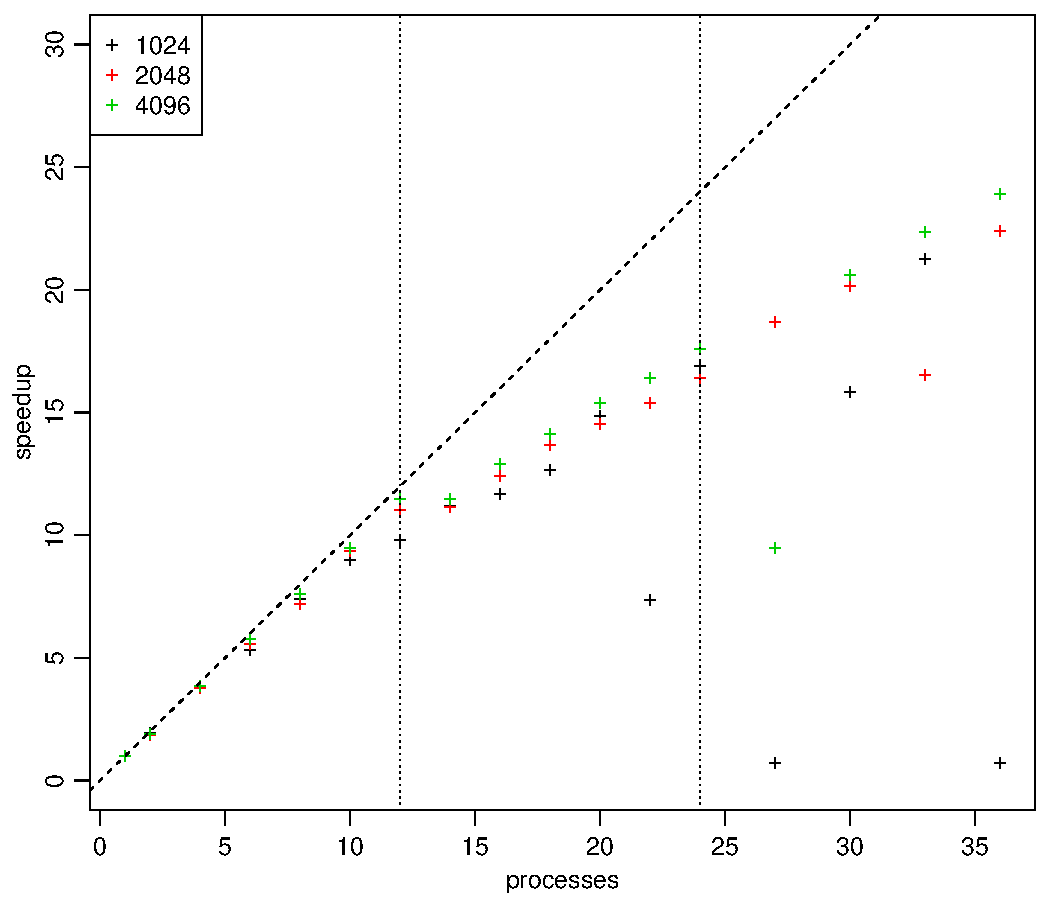
\includegraphics[width=\textwidth]{./Figures/taskbSpeedupProc1.pdf}
  \end{subfigure}%
  \quad
  \begin{subfigure}[b]{0.48\textwidth}
    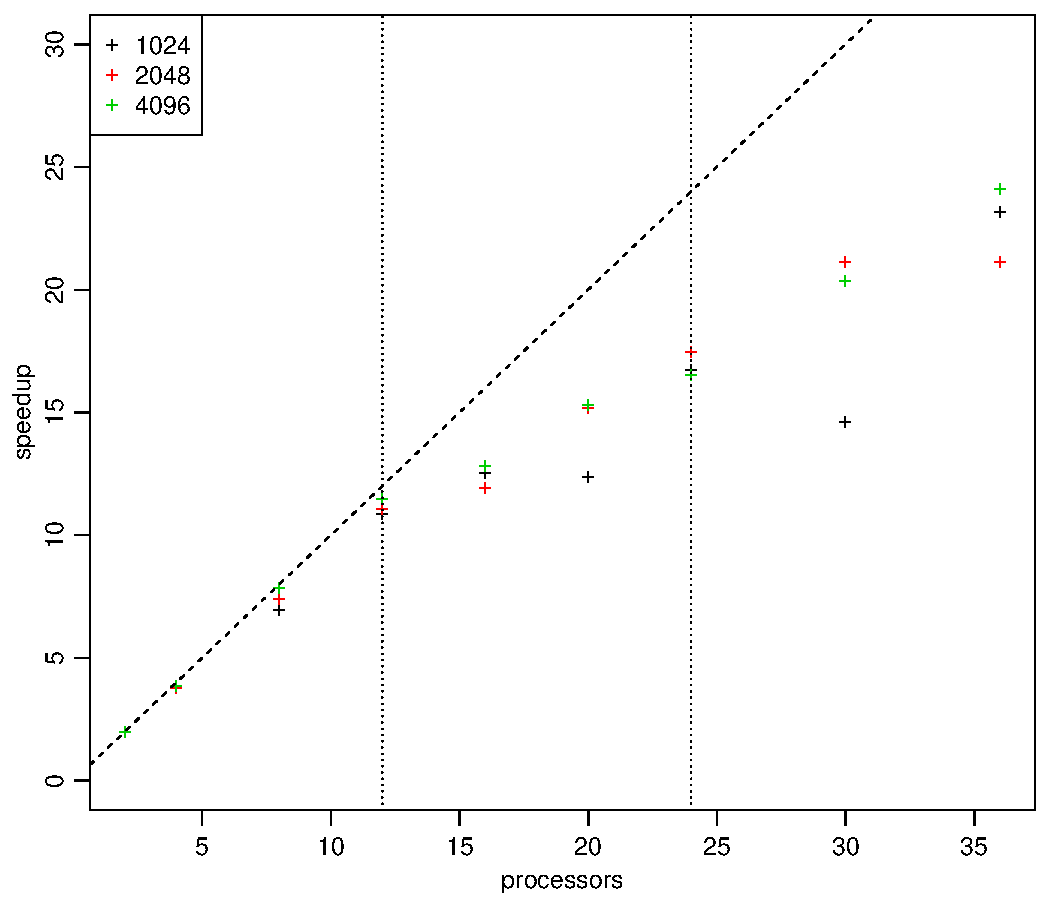
\includegraphics[width=\textwidth]{./Figures/taskbSpeedupProc2.pdf}
  \end{subfigure}
  \quad
  \begin{subfigure}[b]{0.48\textwidth}
    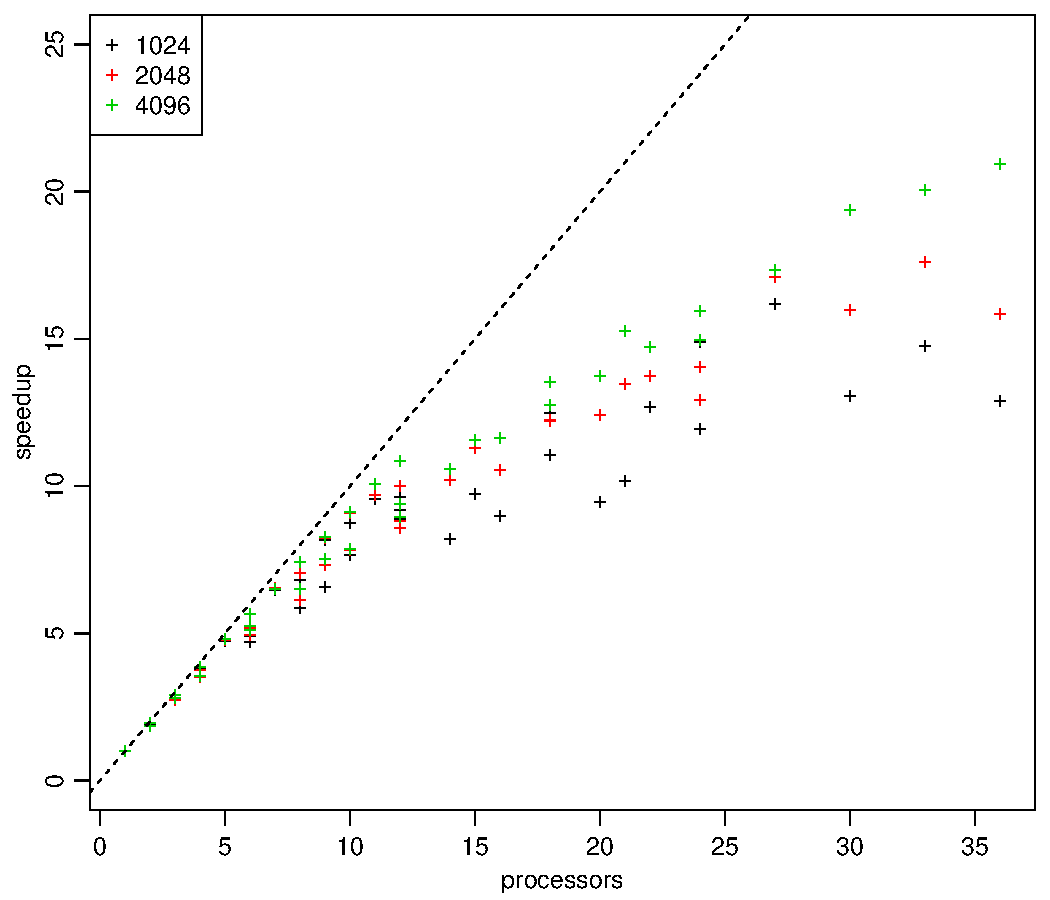
\includegraphics[width=\textwidth]{./Figures/taskbSpeedupNodesTimesThreads.pdf}
  \end{subfigure}
          %(or a blank line to force the subfigure onto a new line)
  \vspace{-0.1\baselineskip}
  \caption{Speedup for running the problem with different amount of MPI processes. In the upper left figure each process has one thread. In the upper right figure each process has two threads. In the bottom figure only one MPI process is run per node and the number of threads varies between 1 and 12. The problem is run on as few nodes as possible, and the MPI processes are identically distributed among the nodes. There are drawn vertical lines to show when a new node is utilized, and a line with slope 1. The green line is the expected speedup from the linear network model \eqref{eq:linNetMod} for $n = 4096$. The problem size $n$ is specified in the plots. }
  \label{fig:Speedup}
\end{figure}
%
\\
The efficiency $\eta = S_p/p $ is another diagnostics tool. this variable will take the value 1 if the speedup is perfect. This is shown in Figure~\ref{fig:Efficiency}. The plots show pretty much the same as Figure~\ref{fig:Speedup}, but the scale is different, so it is easier to see that there is no case of perfect speedup. It is valuable do note that on 1 node the efficiency is around 0.9 and when 2 nodes is used the effiency immediately drops to right below 0.8 and from there it keeps sinking steadily. 
\\
\begin{figure}[h!]
  \centering
  \begin{subfigure}[b]{0.48\textwidth}
    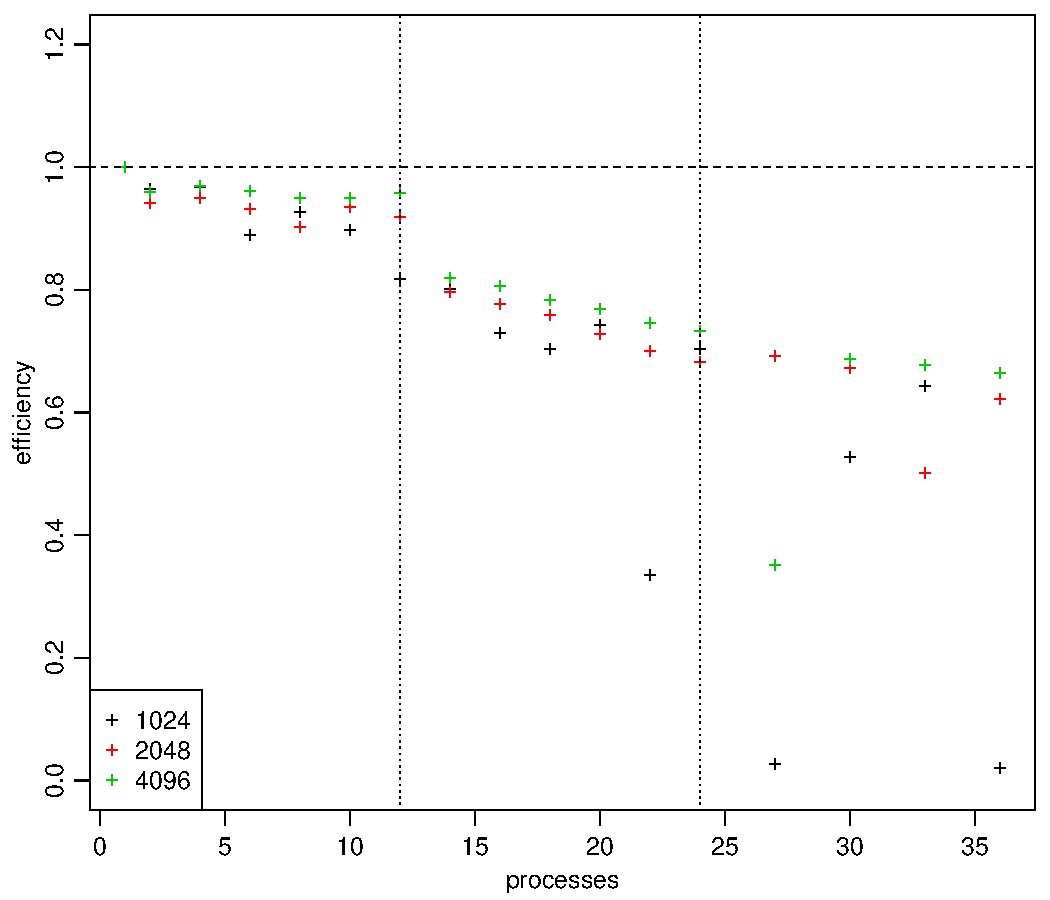
\includegraphics[width=\textwidth]{./Figures/taskbEfficiencyProc1.pdf}
  \end{subfigure}%
  \quad
  \begin{subfigure}[b]{0.48\textwidth}
    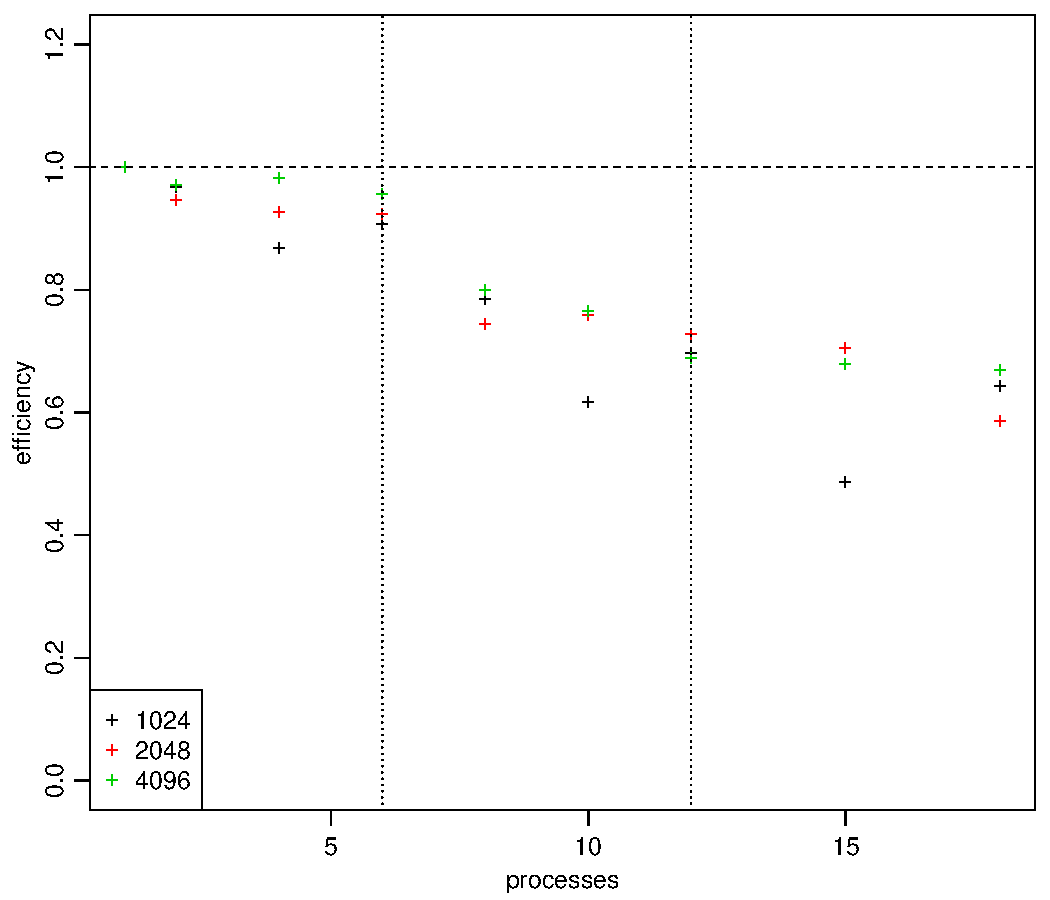
\includegraphics[width=\textwidth]{./Figures/taskbEfficiencyProc2.pdf}
  \end{subfigure}
          %(or a blank line to force the subfigure onto a new line)
  \vspace{-0.1\baselineskip}
	\caption{Efficiency for running problem with different amount of MPI processes. In the left figure each process has one thread. In the right figure each process has two threads. The problem is run on as few nodes as possible, and the MPI processes are identically distributed among the nodes. There are drawn vertical lines to show when a new node is utilized, and a horizontal line at $y=1$. The problem size $n$ is specified in the plots.} 
  \label{fig:Efficiency}
\end{figure}
